\documentclass[sigconf]{acmart}

\usepackage{booktabs} % For formal tables
\usepackage{graphicx}
\definecolor{links}{HTML}{2A1B81}
\hypersetup{colorlinks,linkcolor=,urlcolor=links}
\graphicspath{{./images/} }
% Copyright
\setcopyright{none}
%\setcopyright{acmcopyright}
%\setcopyright{acmlicensed}
%\setcopyright{rightsretained}
%\setcopyright{usgov}
%\setcopyright{usgovmixed}
%\setcopyright{cagov}
%\setcopyright{cagovmixed}


\begin{document}
\title{Conformal Quaternion Based Mesh (Re)Construction}

\author{Adam Sturge}
\orcid{1234-5678-9012}
\affiliation{%
  \institution{Univerity of Toronto}
}
\email{adam.sturge@mail.utoronto.ca}

\acmDOI{0.0/0.0}
\acmISBN{0.0}
\acmPrice{0.00}
\acmConference[CSC2521]{Topics in Computer Graphics: Geometry Processing}{April 2017}{Toronto, Canada} 

% The default list of authors is too long for headers}
\renewcommand{\shortauthors}{A. Sturge}

\begin{abstract}

Mesh (re)construction is the task of building a mesh out of only partial data, most often a point cloud sampling of the implied surface. In this paper we make use of an embedding of $\mathbb{R}^3$ into the quaternions $\mathbb{H}$ to compute  a conformal transformation of a sphere into a target surface. This method differs from other more common techniques in so far as the assumptions made about the target surface are topological instead of geometric. However the tradeoff for these weaker assumptions is a longer runtime compared to traditional algorithms. 

\end{abstract}

\begin{CCSXML}
<ccs2012>
<concept>
<concept_id>10010147.10010371</concept_id>
<concept_desc>Computing methodologies~Computer graphics</concept_desc>
<concept_significance>500</concept_significance>
</concept>
<concept>
<concept_id>10010147.10010371.10010396</concept_id>
<concept_desc>Computing methodologies~Shape modeling</concept_desc>
<concept_significance>300</concept_significance>
</concept>
<concept>
<concept_id>10010147.10010371.10010396.10010397</concept_id>
<concept_desc>Computing methodologies~Mesh models</concept_desc>
<concept_significance>500</concept_significance>
</concept>
</ccs2012>
\end{CCSXML}

\ccsdesc[500]{Computing methodologies~Computer graphics}
\ccsdesc[300]{Computing methodologies~Shape modeling}
\ccsdesc[500]{Computing methodologies~Mesh models}

\keywords{Computer Graphics, Mesh Recontstruction, Conformal Deformation}

\begin{teaserfigure}
\centering
  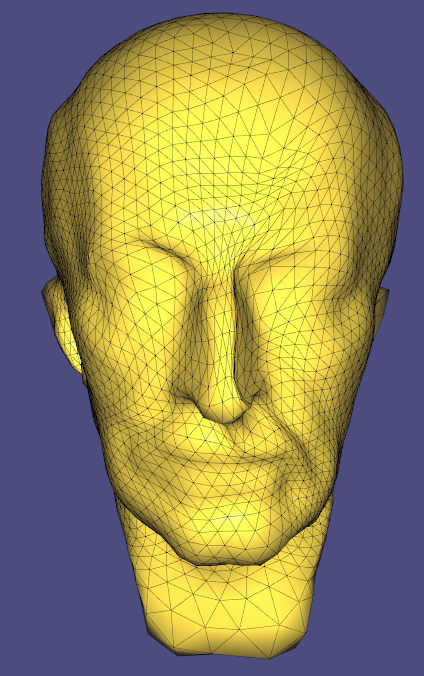
\includegraphics[width=.20\textwidth]{front_sphere_to_head_overnight.PNG}\quad
  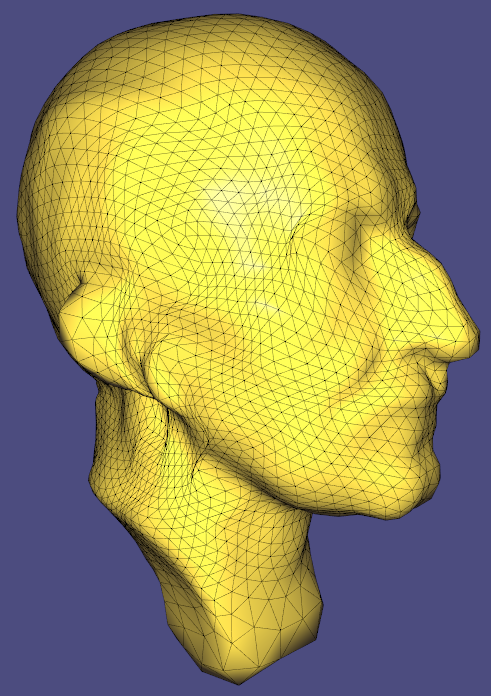
\includegraphics[width=.20\textwidth]{side_sphere_to_head_overnight.PNG}\quad
  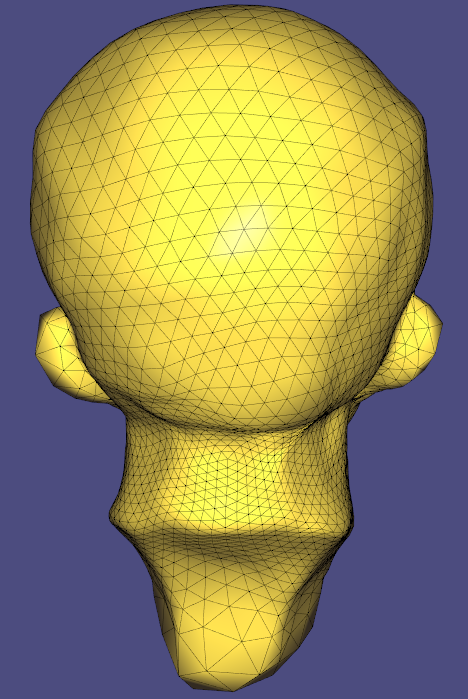
\includegraphics[width=.20\textwidth]{back_sphere_to_head_overnight.PNG}
  \caption{Head mesh generated through conformal quaternion based mesh reconstruction}
  \label{fig:teaser}
\end{teaserfigure}


\maketitle

\section{Links}
\href{https://github.com/AdamSturge/geometry-processing-project}{
\includegraphics[scale=.03]{code-icon.png}}
\hspace{1mm}
\href{https://drive.google.com/open?id=0Bxe_aqElJ61ULXk0S284Y25xME0}{
\includegraphics[scale=.058]{video-play.png}}

\section{Introduction}

Mesh (re)construction is a common problem faced in the video game, animation, and fabrication industries. How to transform a 3D scan of a person or object into a 3D model that can be animated or studied is an important question. Some of the more common ways to deal with this issue are through implict surfaces \cite{Hoppe:2006} or computational geometry \cite{Amenta:2001:PC:376957.376986}.

Here we take the approach of beginning with a seed mesh, one whose topology will be inherited by the final solution. The reasons for pursing this angle are two-fold. First it is not uncommon for someone to have a-priori knowledge of the shape of the target mesh. For example if one knows the scan is of a car then they know the resulting mesh should be car-shaped. From this knowledge it is not unreasonable to take an existing car mesh and deform it to match the 3D scan. Second, even in the case where the user does not know the expected geometry it is generally easy to determine the expected topology from the 3D scan. In this case one can supply a canonical example of the expected topology to transform. 


\section{Related Work: Spin deformation}
In their paper "Spin Transformations of Discrete Surfaces" \cite{Crane:2011:STD} Crane et al develop a method of conformal deformation based on the quaternions. They introduce a discrization of the equation
% Numbered Equation
\begin{equation}
\label{eqn:01}
d\tilde{f} = \bar{\lambda}df\lambda 
\end{equation}
relating the differentials of two surfaces $\tilde{f}$ and $f$ by a quaternion $\lambda$, as well as a sufficient condition for the existence of such a transformation characterized in terms of curvature half density differences between the two surfaces. For our work we will be leaning heavily on these results, specifically the former. The discretization Crane et al discuss leads to the following least squares problem (recalling that quaternion multiplication is not commutative)

\begin{align}
\label{eqn:02}
\tilde{e}_{ij} = \frac{1}{3}\bar{\lambda_{i}}e_{ij}\lambda_{i} + \frac{1}{6}\bar{\lambda_{i}}e_{ij}\lambda_{j} + \frac{1}{6}\bar{\lambda_{j}}e_{ij}\lambda_{i} + \frac{1}{3}\bar{\lambda_{j}}e_{ij}\lambda_{j} \\
\Delta \tilde{f} = \nabla \cdot \tilde{e}
\end{align}
Where $\lambda_{i}$ is a quaternion assigned to vertex $i$ of the original mesh, $e_{ij}$ refers to the edge connecting vertex $i$ to vertex $j$, and $\tilde{f}$ is a vector of the deformed meshes vertices.


\section{Energy Minimization}
\subsection{Energy definition} \label{energy_definition}
In order to transform the seed mesh into the target mesh we need a method to determine how good the fit is. To that end we defined the following two energies, with the goal of minimizing them. 

\begin{equation}
\label{eqn:03}
E(\lambda) = \int_{\Omega}||X(\lambda) - P||^{2}d\Omega \approx \sum_{i=0}^{k}||x_{i}(\lambda) - p_{i}||^{2}
\end{equation}

\begin{equation}
\label{eqn:04}
E(\lambda) = \sum_{i=0}^{k}((x_{i}(\lambda) - p_{i}) \cdot n_{i})^{2}
\end{equation}
Here minimization proceeds in an Iterative Closest Point \cite{Bouaziz:2015} fashion, whereby first we sample $k$ points from the seed mesh and find their closest point in the 3D scan, or vice-versa. The selected energy is then minimized for these points before new points are selected.

The first energy is a simple point-to-point measure of how close each sampled point on the seed mesh $x_{i}(\lambda)$ is to it's closest point in the 3D scan $p_{i}$. The second energy is more relaxed, measuring instead the distance between $x_{i}(\lambda)$ and the plane defined by $p_{i}$ and the normal $n_{i}$. Naturally then this energy requires that the 3D scan also capture an accurate estimate of the normal vector at each point on the surface of the target mesh. However such an assumption isn't an uncommon one \cite{Hoppe:2006}. In practice the choice of which energy to use then comes down to the variety of data we have.

\subsection{Minimization}
By pulling all the quaternions $\lambda_{i}$ into a vector $\vec{\lambda}$ the energies stated in section \ref{energy_definition} can be cast as functionals from $\mathbb{H}^{n}$ to $\mathbb{R}$. Finding a closed form for this minimum is difficult as the relationship between $E$ and $\vec{\lambda}$ is complicated. Instead we opted to go with gradient decent, meaning we iteratively update a best guess by the following rule

\begin{equation}
\label{eqn:05}
\vec{\lambda} \rightarrow \vec{\lambda} + \alpha\frac{\nabla E(\vec{\lambda})}{||\nabla E(\vec{\lambda})||}
\end{equation}
where $\alpha$ is a hyperparameter that controls how far we step in the gradient direction.

\section{Results}
\begin{figure}[htp]
\centering
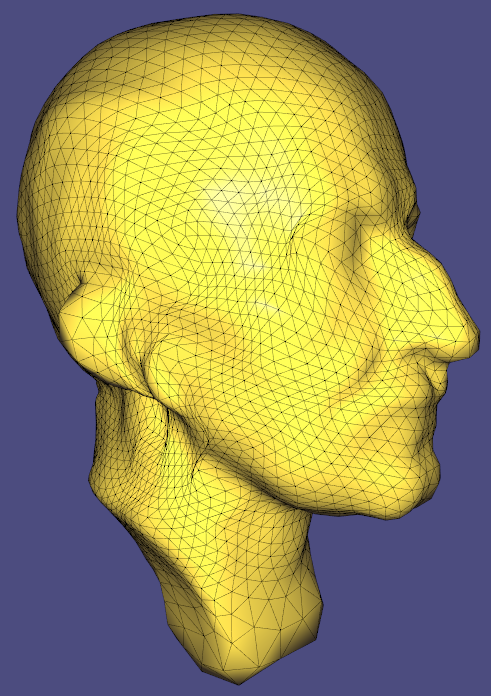
\includegraphics[width=.20\textwidth]{side_sphere_to_head_overnight.PNG}\quad
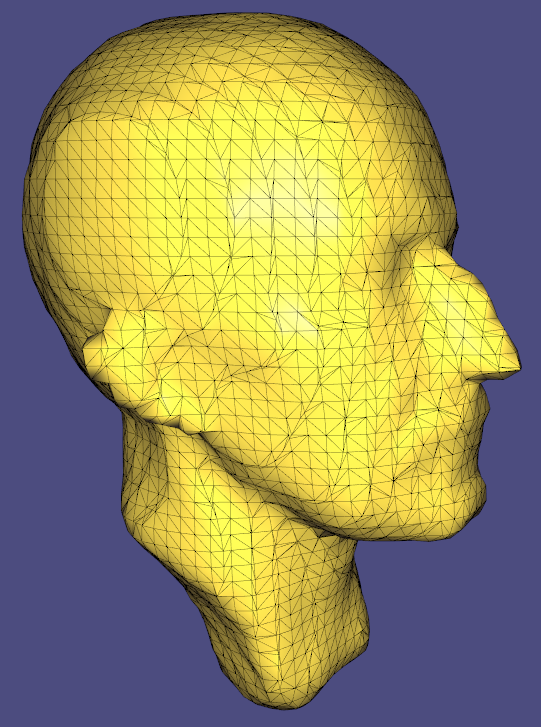
\includegraphics[width=.20\textwidth]{side_poisson.PNG}\quad
\caption{Left : quaternion deformation. Right : Poisson reconstruction assignment}
\label{fig:poisson_comparision}
\end{figure}
One of the benefits and curses of iterative methods is that they can be run continually to produce higher and higher quality meshes. Our technique is doubley iterative as it utilizes both ICP and gradient decent, so this is especially true here. This iterative nature has a large cost in the runtime of our algorithm, taking on the order of 10 minutes to transform a sphere into something resembling a human head. 

Figure \ref{fig:poisson_comparision} shows a comparison of our technique to a naive version of  poisson surface reconstruction \cite{Hoppe:2006} implemented on a fixed spatial grid. The most noticeable difference between the two is the left image has inherited the smoothness of it's seed mesh, whereas the poission mesh has noticeable isolines. However it should also be noted that the possion mesh took seconds to create whereas our method was run overnight.

\section{Conclusion and Future Work}
While we do believe there is some merit to this kind of mesh (re)construction more work needs to be done improving the speed of this technique before it becomes a useful tool. In order of difficulty here are the items the authors feel need to be addressed before anything else.
 
\begin{itemize}
\item Speed up sampling
\item Find a closed form solution for the gradient
\item Find closed form equation for optimal $\vec{\lambda}$ instead of using gradient decent
\end{itemize}

\bibliographystyle{ACM-Reference-Format}
\bibliography{references} 

\end{document}
